\documentclass{standalone}
\usepackage[T1]{fontenc}
\usepackage[latin2]{inputenc}
\usepackage[english]{babel}
\usepackage{tikz}
\usetikzlibrary{calc,through,backgrounds,positioning,fit}
\usetikzlibrary{shapes,arrows,shadows}

\begin{document}

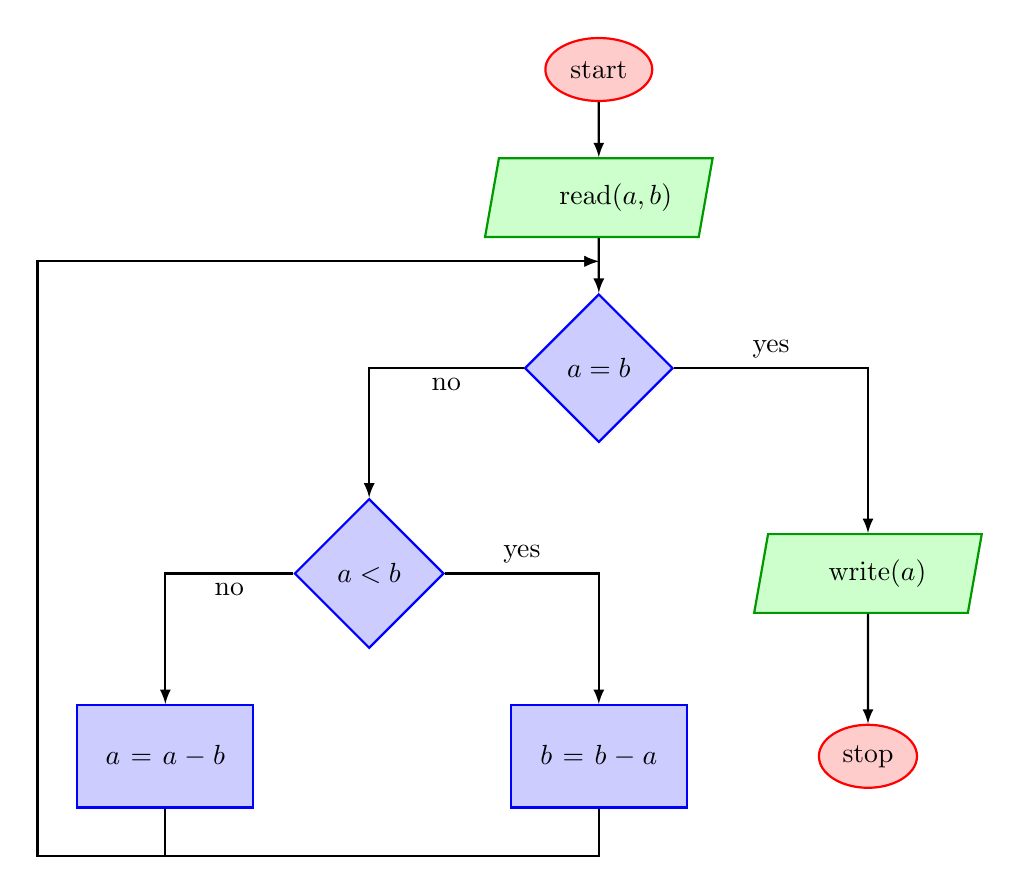
\begin{tikzpicture}[auto,
decision/.style = {diamond, draw=blue, thick, fill=blue!20, text width=1.5cm,
                   align=flush center, inner sep=1pt},
block/.style = {rectangle, draw=blue, thick, fill=blue!20, text width=2cm,
                align=center, minimum height=1.3cm},
start/.style = {draw=red, thick, ellipse, fill=red!20, minimum height=8mm},
inout/.style = {draw=green!60!black, thick, fill=green!20, trapezium, trapezium left angle=80,
                trapezium right angle=-80, minimum height=10mm, text width=1cm, align=center,
                inner sep=1pt},
line/.style ={draw, thick, -latex}]

\coordinate (A) at (-6,-5.5);

\matrix[column sep=5mm,row sep=7mm]
{
% row 1
&& & \node [start] (start) {start}; & \\
% row 2
&& & \node [inout] (read) {read($a,b$)}; & \\
% row 3
&& & \node [decision] (decide_a=b) {$a = b$}; & \\
% row 4
&&  \node [decision] (decide_a<b) {$a < b$}; && \node [inout] (write_a) {write($a$)}; \\
% row 5
& \node [block] (update1) {$a = a - b$}; && \node [block] (update2) {$b = b - a$}; &
  \node [start] (stop) {stop}; \\
};

\begin{scope}[every path/.style=line]
\path (start) -- (read);
\path (read) -- (decide_a=b);
\path (write_a) -- (stop);

\path (decide_a=b) -| node [near start] {yes} (write_a);
\path (decide_a=b) -| node [near start] {no} (decide_a<b);

\path (decide_a<b) -| node [near start] {yes} (update2);
\path (decide_a<b) -| node [near start] {no} (update1);
\path (update1.south) |- (A) |- ($ (decide_a=b.north) + (0,0.4) $);
\path (update2.south) |- (A) |- ($ (decide_a=b.north) + (0,0.4) $);


\end{scope}
\end{tikzpicture}
\end{document}